\section{Metodologia}

O livro \emph{Redes neurais artificiais: teoria e aplicações}\cite{LivroTexto} explica o algoritmo de regularização weight decay
e auxilia sua implementação em redes RBF. A metodologia utilizada define uma variável Lâmbida que representa o termo de penalização do vetor de pesos W.
O efeito do Lâmbida é deslocar a solução do mínimo local da região erro de treinamento com o objetivo de reduzir a absorção de ruído e consequentemente o overfitting.

A regularização foi implementada no algoritmo de treinamento da rede RBF na linguagem python. O código foi feito traduzindo os exemplos em R disponíveis no livro texto e pode ser encontrado no github\footcite{LINK DO GIT} desse trabalho.

\begin{figure}[H]
    \center
    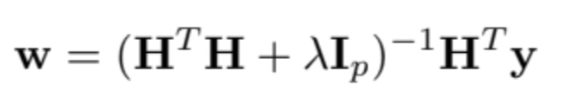
\includegraphics[width=6cm]{images/img9.png}
    \label{img9}
\end{figure}

No algoritmo o vetor de pesos W é influenciado não só pela matriz H que armazena informações do modelo, mas também pela matriz gerada pelo termo de regularização.
Dessa forma, no algoritmo foi adicionado o cálculo da matriz de Variância A, que corresponde ao primeiro termo do cálculo dos pesos W.

\begin{figure}[H]
    \center
    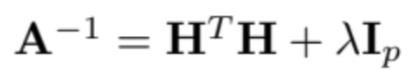
\includegraphics[width=4cm]{images/img10.png}
\end{figure}

O cálculo da Matriz de Projeção P, que será utilizada para cálculo da função Custo J do modelo.

\begin{figure}[H]
    \center
    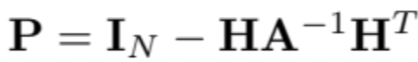
\includegraphics[width=4cm]{images/img11.png}
\end{figure}

Diversos experimentos foram realizados utilizando esse algoritmo de redes RBF para analisar o efeito da regularização. Na próxima seção veremos os resultados.

Para os experimentos utilizando redes Multilayer Perceptron MLP, foram utilizados as bibliotecas prontas para python scikitlearn\cite*[]{scikitlearn}.